%package list
\documentclass{article}
\usepackage[top=3cm, bottom=3cm, outer=3cm, inner=3cm]{geometry}
\usepackage{multicol}
\usepackage{graphicx}
\usepackage{url}
%\usepackage{cite}
\usepackage{hyperref}
\usepackage{array}
%\usepackage{multicol}
\newcolumntype{x}[1]{>{\centering\arraybackslash\hspace{0pt}}p{#1}}
\usepackage{natbib}
\usepackage{pdfpages}
\usepackage{multirow}
\usepackage[normalem]{ulem}
\useunder{\uline}{\ul}{}
\usepackage{svg}
\usepackage{xcolor}
\usepackage{listings}
\lstdefinestyle{ascii-tree}{
    literate={├}{|}1 {─}{--}1 {└}{+}1 
  }
\lstset{basicstyle=\ttfamily,
  showstringspaces=false,
  commentstyle=\color{red},
  keywordstyle=\color{blue}
}
%\usepackage{booktabs}
\usepackage{caption}
\usepackage{subcaption}
\usepackage{float}
\usepackage{array}

\newcolumntype{M}[1]{>{\centering\arraybackslash}m{#1}}
\newcolumntype{N}{@{}m{0pt}@{}}


%%%%%%%%%%%%%%%%%%%%%%%%%%%%%%%%%%%%%%%%%%%%%%%%%%%%%%%%%%%%%%%%%%%%%%%%%%%%
%%%%%%%%%%%%%%%%%%%%%%%%%%%%%%%%%%%%%%%%%%%%%%%%%%%%%%%%%%%%%%%%%%%%%%%%%%%%
\newcommand{\itemEmail}{fayamamani@unsa.edu.pe}
\newcommand{\itemStudent}{Francis Willian Ayamamani Añasco}
\newcommand{\itemCourse}{Programación Web 2}
\newcommand{\itemCourseCode}{GUIA-PRLD-001}
\newcommand{\itemSemester}{I}
\newcommand{\itemUniversity}{Universidad Nacional de San Agustín de Arequipa}
\newcommand{\itemFaculty}{Facultad de Ingeniería de Producción y Servicios}
\newcommand{\itemDepartment}{Departamento Académico de Ingeniería de Sistemas e Informática}
\newcommand{\itemSchool}{Escuela Profesional de Ingeniería de Sistemas}
\newcommand{\itemAcademic}{2023 - A}
\newcommand{\itemInput}{Del 5 Junio 2023}
\newcommand{\itemOutput}{Al 5 Junio 2023}
\newcommand{\itemPracticeNumber}{01}
\newcommand{\itemTheme}{Vim - Git - GitHub}
%%%%%%%%%%%%%%%%%%%%%%%%%%%%%%%%%%%%%%%%%%%%%%%%%%%%%%%%%%%%%%%%%%%%%%%%%%%%
%%%%%%%%%%%%%%%%%%%%%%%%%%%%%%%%%%%%%%%%%%%%%%%%%%%%%%%%%%%%%%%%%%%%%%%%%%%%

\usepackage[english,spanish]{babel}
\usepackage[utf8]{inputenc}
\AtBeginDocument{\selectlanguage{spanish}}
\renewcommand{\figurename}{Figura}
\renewcommand{\refname}{Referencias}
\renewcommand{\tablename}{Tabla} %esto no funciona cuando se usa babel
\AtBeginDocument{%
	\renewcommand\tablename{Tabla}
}

\usepackage{fancyhdr}
\pagestyle{fancy}
\fancyhf{}
\setlength{\headheight}{30pt}
\renewcommand{\headrulewidth}{1pt}
\renewcommand{\footrulewidth}{1pt}
\fancyhead[L]{\raisebox{-0.2\height}{
\includegraphics[width=3cm]{img/logo_episunsa.png}}}
\fancyhead[C]{\fontsize{7}{7}\selectfont	\itemUniversity \\ \itemFaculty \\ \itemDepartment \\ \itemSchool \\ \textbf{\itemCourse}}
\fancyhead[R]{\raisebox{-0.2\height}{
\includegraphics[width=1.2cm]{img/logo_abet}}}
\fancyfoot[L]{Estudiante Francis Ayamamani Añasco}
\fancyfoot[C]{\itemCourse}
\fancyfoot[R]{Página \thepage}

% para el codigo fuente
\usepackage{listings}
\usepackage{color, colortbl}
\definecolor{dkgreen}{rgb}{0,0.6,0}
\definecolor{gray}{rgb}{0.5,0.5,0.5}
\definecolor{mauve}{rgb}{0.58,0,0.82}
\definecolor{codebackground}{rgb}{0.95, 0.95, 0.92}
\definecolor{tablebackground}{rgb}{0.8, 0, 0}

\lstset{frame=tb,
	language=bash,
	aboveskip=3mm,
	belowskip=3mm,
	showstringspaces=false,
	columns=flexible,
	basicstyle={\small\ttfamily},
	numbers=none,
	numberstyle=\tiny\color{gray},
	keywordstyle=\color{blue},
	commentstyle=\color{dkgreen},
	stringstyle=\color{mauve},
	breaklines=true,
	breakatwhitespace=true,
	tabsize=3,
	backgroundcolor= \color{codebackground},
}

\begin{document}
	
	\vspace*{10px}
	
	\begin{center}	
		\fontsize{17}{17} \textbf{ Informe de Laboratorio \itemPracticeNumber}
	\end{center}
	\centerline{\textbf{\Large Tema: \itemTheme}}
	%\vspace*{0.5cm}	

	\begin{flushright}
		\begin{tabular}{|M{2.5cm}|N|}
			\hline 
			\rowcolor{tablebackground}
			\color{white} \textbf{Nota}  \\
			\hline 
			     \\[30pt]
			\hline 			
		\end{tabular}
	\end{flushright}	

	\begin{table}[H]
		\begin{tabular}{|x{4.7cm}|x{4.8cm}|x{4.8cm}|}
			\hline 
			\rowcolor{tablebackground}
			\color{white} \textbf{Estudiante} & \color{white}\textbf{Escuela}  & \color{white}\textbf{Asignatura}   \\
			\hline 
			{\itemStudent \par \itemEmail} & \itemSchool & {\itemCourse \par Semestre: \itemSemester \par Código: \itemCourseCode}     \\
			\hline 			
		\end{tabular}
	\end{table}		
	
	\begin{table}[H]
		\begin{tabular}{|x{4.7cm}|x{4.8cm}|x{4.8cm}|}
			\hline 
			\rowcolor{tablebackground}
			\color{white}\textbf{Laboratorio} & \color{white}\textbf{Tema}  & \color{white}\textbf{Duración}   \\
			\hline 
			\itemPracticeNumber & \itemTheme & 04 horas   \\
			\hline 
		\end{tabular}
	\end{table}
	
	\begin{table}[H]
		\begin{tabular}{|x{4.7cm}|x{4.8cm}|x{4.8cm}|}
			\hline 
			\rowcolor{tablebackground}
			\color{white}\textbf{Semestre académico} & \color{white}\textbf{Fecha de inicio}  & \color{white}\textbf{Fecha de entrega}   \\
			\hline 
			\itemAcademic & \itemInput &  \itemOutput  \\
			\hline 
		\end{tabular}
	\end{table}
	
	\section{Tarea}
	\begin{itemize}		
		\item Crear repositorio GitHub.
        \item Instalar Git
        \begin{itemize}
            \item sudo apt-get update
		      \item sudo apt-get install git
		      \item password:usuario
        \end{itemize}
\item Crear un directorio pw2-lab-d-23a en cualquier sitio.
\item Dentro de este directorio inicializar un repositorio.
\begin{itemize}
    \item git config --global user.name "Richart Escobedo Quispe"
	\item git config --global user.email rescobedoq@unsa.edu.pe
	\item git init
	\item git branch -M main
\end{itemize}
\item Empezar a crear una página de acuerdo al Tutorial de la W3C.
\begin{itemize}
    \item Agregar contenido personalizado por ud.
	\item Agregar fotos.
    \item URL: https://www.w3.org/Style/Examples/011/firstcss.es.html 
\end{itemize}

\item Sincronizar Git en Github (Repetir cuantas veces quieres commitear	)
		\begin{itemize}
		    \item git add .
            \item git commit -m "Envío index.html Plantilla inicial"
		      \item git remote add origin HTTTPS-GITHUB-URL
		      \item git push -u origin main
		      \item username o email: rescobedoq@unsa.edu.pe
		      \item password: PERSONAL-TOKEN
		\end{itemize}
	\end{itemize}
		
	\section{MARCO CONCEPTUAL}
	\begin{itemize}
		\item Editor Vim
        \begin{itemize}
            \item Vim es un editor de texto muy eficiente para programar en consola que no tiene nada que envidiar a los editores gráficos.
        \end{itemize}
        \item Instalar Vim en
        \begin{itemize}
            \item GNU/Linux
            \begin{itemize}
                \begin{verbatim}
                    apt-get install vim
                \end{verbatim}
            \end{itemize}
            \item MS Windows
            \begin{itemize}
                \item Para descarga en sistemas MS Windows https://www.vim.org/download.php
            \end{itemize}
            \item MacOS
            \begin{itemize}
                \begin{verbatim}
                    brew install macvim
                \end{verbatim}
            \end{itemize}
        \end{itemize}
        \item Git
        \begin{itemize}
            \item Git es un sistema de control de versiones creado por Linus Torvalds. Es eficiente, confiable.
        \end{itemize}
        \item Instalar Git
        \begin{itemize}
            \item GNU/Linux
            \begin{itemize}
                \begin{verbatim}
                    apt-get install git
                \end{verbatim}
            \end{itemize}
            \item MS Windows
            \begin{itemize}
                \item Para descarga en sistemas MS Windows https://git-scm.com/download/win
            \end{itemize}
            \item MacOS
            \begin{itemize}
                \item Para descarga en sistemas MacOS https://git-scm.com/download/mac
                \begin{verbatim}
                    brew install git
                \end{verbatim}
            \end{itemize}
        \end{itemize}
	\end{itemize}
	
	\section{URL de Repositorio Github}
	\begin{itemize}
		\item URL del Repositorio GitHub para clonar o recuperar.
		\item \url{https://github.com/rescobedoq/programacion.git}
		\item URL para el laboratorio 01 en el Repositorio GitHub.
		\item \url{https://github.com/rescobedoq/programacion/tree/main/lab01}
	\end{itemize}
	
	\section{Resolucion de la tarea}
	
	\subsection{Crear repositorio GitHub}
	\begin{itemize}	
		\item Como es el primer laboratorio se creo el repositorio GitHub.
		\item Se realizaron los siguientes comandos en la computadora:
	\end{itemize}	
		
	\begin{lstlisting}[language=bash,caption={Creando directorio de trabajo}][H]
		$ mkdir $HOME/francis/pw2-lab-d-23a
	\end{lstlisting}
	\begin{lstlisting}[language=bash,caption={Dirijíéndonos al directorio de trabajo}][H]
		$ cd $HOME/francis/pw2-lab-d-23a
	\end{lstlisting}	
	\begin{lstlisting}[language=bash,caption={Inicializando directorio para repositorio GitHub}][H]
		$ cd $HOME/francis/pw2-lab-d-23a/programacion
		$ git init
		$ git config --global user.name "Francis Willian Ayamamani"
		$ git config --global user.email fayamamani@unsa.edu.pe
		$ git commit -m "Inicializando la carpeta de trabajo"
		$ git branch -M main
		$ git remote add origin https://github.com/WillianAyamamani/pw2-lab-d-23a
		$ git push -u origin main
	\end{lstlisting}
	
	\subsection{Commits}
    \begin{lstlisting}[language=bash, caption={Creando index.html}][H]
    $ vim index.html
    \end{lstlisting}
    \begin{figure}[H]
		\centering
		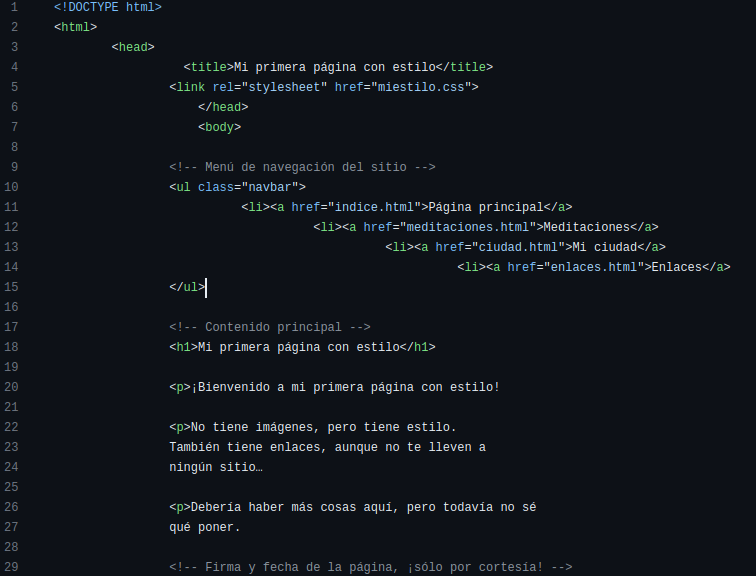
\includegraphics[width=0.8\textwidth,keepaspectratio]{img/index1.png}
		%\includesvg{img/automata.svg}
		%\label{img:mot2}
		%\caption{Product backlog.}
	\end{figure}
    \begin{figure}[H]
		\centering
		
\includegraphics[width=0.8\textwidth,keepaspectratio]{img/index2.png}
		%\includesvg{img/automata.svg}
		%\label{img:mot2}
		%\caption{Product backlog.}
	\end{figure}
    \begin{lstlisting}[language=bash, caption={Creando inicio.html}][H]
    $ vim inicio.html
    \end{lstlisting}
    \begin{figure}[H]
		\centering
		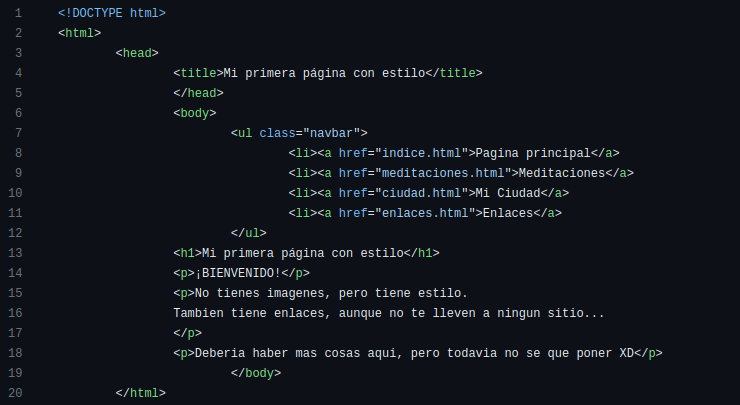
\includegraphics[width=0.8\textwidth,keepaspectratio]{img/inicio.png}
		%\includesvg{img/automata.svg}
		%\label{img:mot2}
		%\caption{Product backlog.}
	\end{figure}
    \begin{lstlisting}[language=bash, caption={Creando miestilo.css}][H]
    $ vim miestilo.css
    \end{lstlisting}
    \begin{figure}[H]
		\centering
		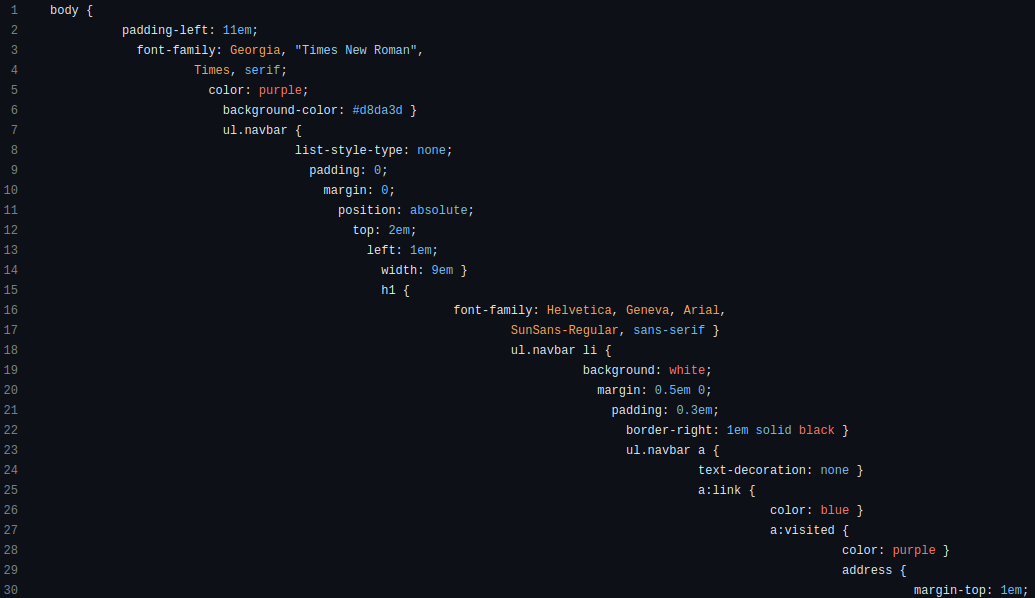
\includegraphics[width=0.8\textwidth,keepaspectratio]{img/estilo.png}
		%\includesvg{img/automata.svg}
		%\label{img:mot2}
		%\caption{Product backlog.}
	\end{figure}
	\begin{lstlisting}[language=bash,caption={Corrigiendo directorio general}][H]
		$ mkdir lab1
		$ mv index.html miestilo.css inicio.html /lab1
		$ git add .
		$ git commit -m "Corrigiendo directorio general"			
		$ git push -u origin main
	\end{lstlisting}
	\subsection{Estructura de laboratorio 01}
	\begin{itemize}	
		\item El contenido que se entrega en este laboratorio es el siguiente:
	\end{itemize}
	
\begin{lstlisting}[style=ascii-tree]
lab01/
|--- inicio.html
|--- index.html
|--- miestilo.css
|--- latex
    |--- img
    |   |--- logo_abet.png
    |   |--- index.png
    |   |--- inicio.png
    |   |--- estilo.png
    |   |--- logo_episunsa.png
    |   |--- logo_unsa.jpg
    |   |--- pseudocodigo_insercion.png    
    |--- lab1.pdf    
    |--- lab1.tex
\end{lstlisting}    

\section{Cuestionario}
	\begin{itemize}
		\item ¿Por qué Git y GitHub son herramientas importantes para el curso?
        \begin{itemize}
           \item Git y GitHub son herramientas esenciales para el curso, ya que brindan a los estudiantes la capacidad de trabajar de manera colaborativa, rastrear los cambios en el código fuente y utilizar características adicionales para mejorar su flujo de trabajo y mostrar sus proyectos de manera efectiva.
        \end{itemize}
        \item ¿Qué conductas éticas deberían promocionarse cuando se usa un Sistema de Control de Versiones?
        \begin{itemize}
           \item Respeto a la propiedad intelectual,Colaboración transparente,Respeto a las políticas del proyecto,Reconocimiento y atribución. Al promover estas conductas éticas, se fomenta un entorno de trabajo colaborativo, respetuoso y responsable en el uso de un Sistema de Control de Versiones.
        \end{itemize}
        \item ¿Qué son los entándares de codificación?
        \begin{itemize}
           \item Los estándares de codificación son conjuntos de pautas y reglas establecidas para garantizar la consistencia y legibilidad del código fuente en un proyecto de desarrollo de software. Estos estándares definen un conjunto común de convenciones y prácticas que los desarrolladores deben seguir al escribir código.
        \end{itemize}
	\end{itemize}		

	\section{\textcolor{red}{Rúbricas}}
	
	\subsection{\textcolor{red}{Entregable Informe}}
	\begin{table}[H]
		\caption{Tipo de Informe}
		\setlength{\tabcolsep}{0.5em} % for the horizontal padding
		{\renewcommand{\arraystretch}{1.5}% for the vertical padding
		\begin{tabular}{|p{3cm}|p{12cm}|}
			\hline
			\multicolumn{2}{|c|}{\textbf{\textcolor{red}{Informe}}}  \\
			\hline 
			\textbf{\textcolor{red}{Latex}} & \textcolor{blue}{El informe está en formato PDF desde Latex,  con un formato limpio (buena presentación) y facil de leer.}   \\ 
			\hline 
			
			
		\end{tabular}
	}
	\end{table}
	
	\clearpage
	
	\subsection{\textcolor{red}{Rúbrica para el contenido del Informe y demostración}}
	\begin{itemize}			
		\item El alumno debe marcar o dejar en blanco en celdas de la columna \textbf{Checklist} si cumplio con el ítem correspondiente.
		\item Si un alumno supera la fecha de entrega,  su calificación será sobre la nota mínima aprobada, siempre y cuando cumpla con todos lo items.
		\item El alumno debe autocalificarse en la columna \textbf{Estudiante} de acuerdo a la siguiente tabla:
	
		\begin{table}[ht]
			\caption{Niveles de desempeño}
			\begin{center}
			\begin{tabular}{ccccc}
    			\hline
    			 & \multicolumn{4}{c}{Nivel}\\
    			\cline{1-5}
    			\textbf{Puntos} & Insatisfactorio 25\%& En Proceso 50\% & Satisfactorio 75\% & Sobresaliente 100\%\\
    			\textbf{2.0}&0.5&1.0&1.5&2.0\\
    			\textbf{4.0}&1.0&2.0&3.0&4.0\\
    		\hline
			\end{tabular}
		\end{center}
	\end{table}	
	
	\end{itemize}
	
	\begin{table}[H]
		\caption{Rúbrica para contenido del Informe y demostración}
		\setlength{\tabcolsep}{0.5em} % for the horizontal padding
		{\renewcommand{\arraystretch}{1.5}% for the vertical padding
		%\begin{center}
		\begin{tabular}{|p{2.7cm}|p{7cm}|x{1.3cm}|p{1.2cm}|p{1.5cm}|p{1.1cm}|}
			\hline
    		\multicolumn{2}{|c|}{Contenido y demostración} & Puntos & Checklist & Estudiante & Profesor\\
			\hline
			\textbf{1. GitHub} & Hay enlace URL activo del directorio para el  laboratorio hacia su repositorio GitHub con código fuente terminado y fácil de revisar. &2 &X &2 & \\ 
			\hline
			\textbf{2. Commits} &  Hay capturas de pantalla de los commits más importantes con sus explicaciones detalladas. (El profesor puede preguntar para refrendar calificación). &4 & & & \\ 
			\hline 
			\textbf{3. Código fuente} &  Hay porciones de código fuente importantes con numeración y explicaciones detalladas de sus funciones. &2 &X &2 & \\ 
			\hline 
			\textbf{4. Ejecución} & Se incluyen ejecuciones/pruebas del código fuente  explicadas gradualmente. &2 &X &2 & \\ 
			\hline			
			\textbf{5. Pregunta} & Se responde con completitud a la pregunta formulada en la tarea.  (El profesor puede preguntar para refrendar calificación).  &2 &X &2 & \\ 
			\hline	
			\textbf{6. Fechas} & Las fechas de modificación del código fuente estan dentro de los plazos de fecha de entrega establecidos. &2 &X &2 & \\ 
			\hline 
			\textbf{7. Ortografía} & El documento no muestra errores ortográficos. &2 &X &2 & \\ 
			\hline 
			\textbf{8. Madurez} & El Informe muestra de manera general una evolución de la madurez del código fuente,  explicaciones puntuales pero precisas y un acabado impecable.   (El profesor puede preguntar para refrendar calificación).  &4 & & & \\ 
			\hline
			\multicolumn{2}{|c|}{\textbf{Total}} &20 & &12 & \\ 
			\hline
		\end{tabular}
		%\end{center}
		%\label{tab:multicol}
		}
	\end{table}
	
\clearpage

\section{Referencias}
\begin{itemize}			
	\item \url{https://www.w3schools.com/java/default.asp}
	\item \url{https://www.geeksforgeeks.org/insertion-sort/}
\end{itemize}	
	
%\clearpage
%\bibliographystyle{apalike}
%\bibliographystyle{IEEEtranN}
%\bibliography{bibliography}
			
\end{document}
